\subsection{Introduction}
The modelation of Cities as 3D City model got more famous in the last years. Different appraoches from different domains to model the real world are common. The most famous domains, which deal with the creation of 3D models are Computer graphics, Architectural aided design and geoinformation science. In computer graphic and architecturel models only the geometry is represented. 3D models in geoinformation science store next to the geometry also semantics. This enables a user to use the 3D models for further investigations. This project deals with the enrichment of such a city model with an additional semantic layer, which contains energy related attributes. For this, the data of the 3D City DB of Berlin Moabit is used. Because the buildings are only available in LoD2, although LoD3 is required for a reliable energy demand estimation first LoD3 buildings are modeled. To create LoD 3 buildings different approach to model 3D building models with from building photographs are adopted. SketchUP is used for the 
modelation process. These models are enriched with the mentioned energy related attributes. Finally the new LoD 3 models are integrated in the 3D City DB.

\subsection{Workflow}
To model LoD 3 buildings and enrich them with energy realted attributes, the work can be splitted in three main parts, data acquisistion, 3D modeling and data integration. Figure \ref{fig:workflowph1} depicts the content of each project phase.

\begin{figure}[ht]
	\centering
	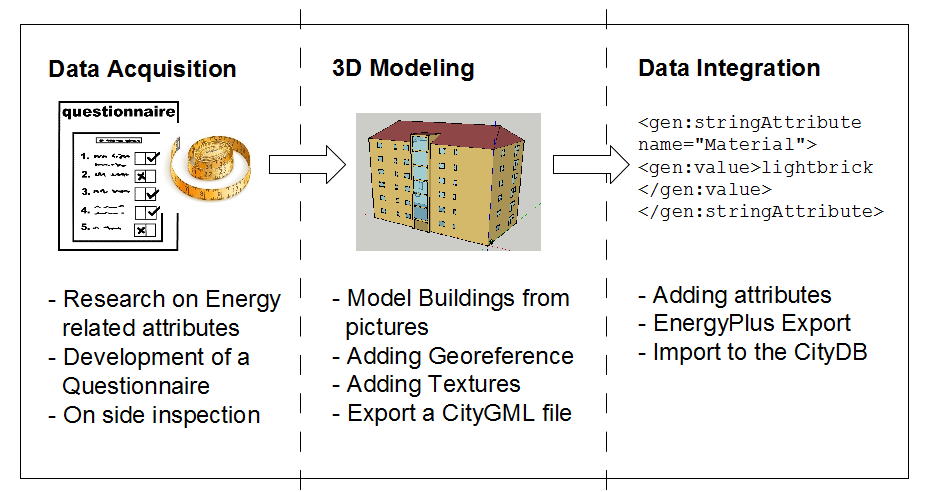
\includegraphics[width=0.8\textwidth]{phase1/group2/figures/workflow_phase1.png}
	\caption{Work packages for phase 1 of the GIS project}
	\label{fig:workflowph1}
\end{figure}

To model a LoD 3 building additional information about the geometry of e.g. windows, doors, as well as high resolution textures are necessary. For the integration of energy related attributes additional semantic data like the number of flats or the heating system have to be aquired. In order to collect this data a questionnaire was developed in the first step. \\
These questionnaire was used to acquire the necssary data for individual buildings by an onsite inspection. \\
The collected data is used to create LoD 3 models with SketchUP in phase 2. 
\\
Finally the models are enriched with the energy related attributes that are needed for the objective of this project.
Furthermore the new 3D models are exported as CityGML files and integrated into the 3D City Database. \\
In addition it was tried to export the building models as Energy Plus files, in order to run a Energy simulation with different input parameters. Because several problems with the SketchUp plugin Open Studio, which provides functions to generate Energy Plus consistent building models, were encountered it was not possible to export a Energy Plus file. \\
Therefore the report concentrates on the development of LoD 3 building models. 
\\
From the work packages the project schedule was created as guide to manage the project within a specific time frame. The project schedule can be found in annex1

\subsection{Data acquisistion}
\subsubsection{Development of a questionnaire}
The questionnare should cover all relevant questions to collect the data, which is needed for the creation of LoD 3 buildings models and the enrichment of these with energy related attributes. Therefore the requirments for LoD 3 building models have to be known. A LoD 3 building geometry comprises surface as well as windows, doors and balconies. Furthermore high resolution textures have to be available. To decide which energy related attributes are neccessary the "Kurzverfahren Energie Profil" of the Institut fuer Wohnen und Umwelt (IWU 2003) was used as reference. The questionnare can be seperated into eight parts:
\begin{itemize}
\item Address
\item General building attributes: Year of Construction, Number of flats, functionality, etc. (Figure \ref{fig:questionnaire}
\item Ground plan: sketch to get a better orientation
\item Adjacent buildings: neighboorhood sitiuation of the building (free standing, neighboor)
\item Basement
\item Roof: type, material, etc.
\item Window: Number of windows, U-values
\item Walls: Type, Insolation, Thickness, etc.
\item Doors: Material
\item Heating system
\item Additional notes
\end{itemize}

To simplify the field work for most questions predefined choices were created. For example seven roof types are proposed. The whole questionaire can be found in annex 2.

\begin{figure}[ht]
	\centering
	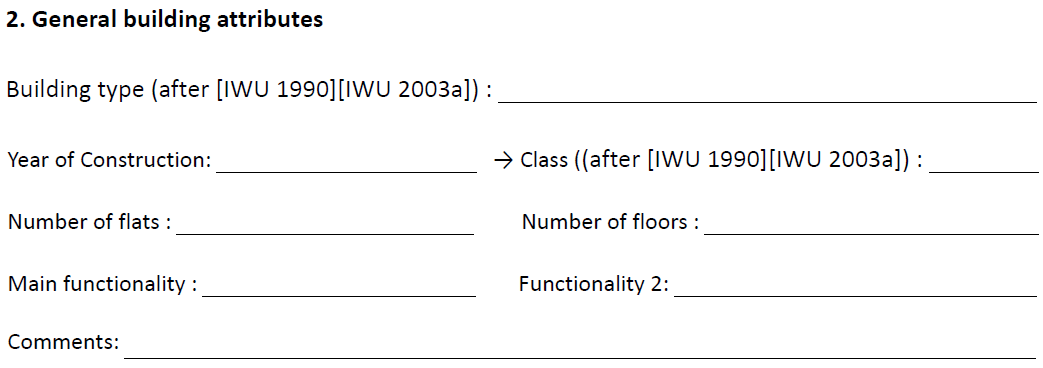
\includegraphics[width=0.8\textwidth]{phase1/group2/figures/questionnaire.png}
	\caption{Developed questionnaire}
	\label{fig:questionnaire}
\end{figure}


\subsubsection{Onsite inspection and data acquisistion}

The area of interest of the project is Berlin Moabit. In this area six buildings were selected based on different criteria like functionality, neighboring situation and year of construction. Therefore one free standing young office building, one old (1961) residential building with two adjacent buildings, as well as three residential buildings with one adjacent building were selected. \\
For this six buildings the questionnare was answered and several images were taken. Additionaly measuremnts were performed to determine the thickness of the walls and at least one reference height in order to scale the building models correctly. 
The images are later on used to model the buildings. Therefore images of each corner and each surface have to be taken as shown in figure \ref{fig:images}.

\begin{figure}[ht]
	\centering
	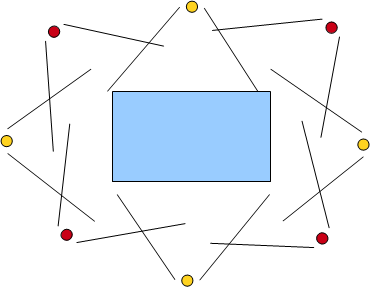
\includegraphics[width=0.5\textwidth]{phase1/group2/figures/images.png}
	\caption{Constrains on image acquisition}
	\label{fig:images}
\end{figure}

Because most of the buildings have adjacent buildings it was not always possible to take proper images of the building corners. Furthermore trees and cars were in the field of view.\\
The questionnaire is very detailed and covers all necessary data. In reality it has to be admitted that it was not possible to gather all information proposed by the questionnaire. For example it was only possible to collect information about the heating system for one building. The determination of year of construction of the buildings was not accuratly, too. The gathered information about the roof, e.g. type and material, the windows and doors, e.g. glazing, and walls is reliable.
\\
\\
The collected data is reorganized for furhter processings in a new Data sheet. It is attached as annex 3.

\subsection{3D Modeling}
The creation of LoD 3 building models is the major part of this project phase. To model the building SketchUp, a 3D modeling software, is used. In addition several SketchUP plugins such as Geores, a plugin to export the SketchUP models to CityGML, or OpenStudio, a plugin to generate Energy plus convienent models, are used. Furthermore FME is used to attach attributes to the CityGML models. The 3D City DB Importer and Exporter tool, which was developed by the geodesy and Geoinformation department of the Technical University of Berlin, is used to validate the created CityGML files and to integrate them in the 3D City DB.

\subsubsection{Creation of building model}
The 3D building modeling is based on the acquired images from different perspectives.To model consistent LoD3 buildings a work pattern was development, which was followed for all buildings. In the following the single steps are pointed out.
 
\begin{itemize}
\item Definition of left and right vanishing points.
\item Photos are calibrated based on the assumption that there are 90° angles.
\item Set the origin to a corner of the building. 
\item Set the scale. This is done by drawing a line representing the measured reference distance and scaling it to the real world length. Reference distances are measurments of the door, window or the 2D foot print which is extracted from the existing LoD 2 model in the 3D City DB.
\item Digitize the shape of the building from the current image as far as possible.Continue with the next images in the same way.
\item Windows and doors are digitized by creating openings in the. 
\end{itemize}

The roof of the building cannot be created from the acquired images. The shapes of the roofs are estimated from the satellite images of google earth and modeleld without reference.

\begin{figure}[ht]
	\centering
	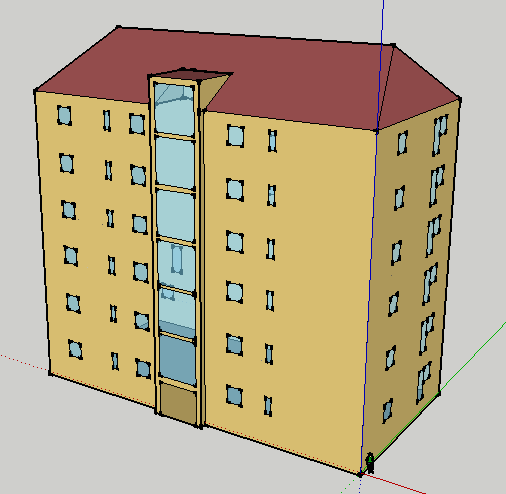
\includegraphics[width=0.5\textwidth]{phase1/group2/figures/Building_wiclef.png}
	\caption{Work packages for phase 1 of the GIS project}
	\label{fig:Building_wiclef}
\end{figure}

After the creation of the 3D model of a building the used images are projected on the surface of the models and used as textures. Because some images are highly distorted the textures don't correspond perfectly to the geometry. The following steps were followed to project the texture on the model.

\begin{itemize}
\item choose a picture
\item Mark the surface to which the texture should be applied 
\item Press the buttion "project texture from photos" from the "Match-Photo"-Dialog
\end{itemize}

Four of the six buildings were modeled with this workflow.


\subsubsection{Handling Layers in SketchUP}

For a successful export to cityGML the features of a building have to organized in a sophisticated layer structure.
Different layers are created for the model in order to identify each surface and opening as a unique entity in the exported cityGML file. The layer is created with sketch up following some standard rules to make each layer unique with an id. The workflow used for creating the layers is as follows:


\begin{itemize}
\item Highlighted a particular surface or part of the building model 
\item Click on ``create layer'' from the window button in sketch up
\item Assign a layer name according to following rules
\end{itemize}

This is repeated for all the surfaces and all the building part of the model. Features of each surface could be grouped or ungrouped for a single surface. For the purpose of this project the building features are mostly grouped. 

To make the model compatible to the GEORES plugin of sketch up, the layer need to named according to some rules which will be explained in the following chapter.
All layers belonging to one building need to start with the same prefix, followed by a dot.
\begin{lstlisting}
building1.
\end{lstlisting}

For each wall, ground or roof surface an extra layer has to be created as subitems of the building and the given ids of the surfaces have to unique within the model.
\begin{lstlisting}
building1.wall1
building1.roof1
building1.ground1
\end{lstlisting}
 Surfaces belonging to one type can also be assigned to one layer, but they need to be grouped instead of the id,  a "s" indicates that there are grouped surfaces in the layer.  If a surface has subsurfaces (openings) like windows or doors it cannot be grouped and needs to be in an extra layer as shown above.
 \begin{lstlisting}
  building1.walls
building1.roofs
building1.grounds
 \end{lstlisting}

Openings must be either a door or windows and the layer name follows the same schema.
A unique id for each opening, or openings belonging to one surface can be grouped and assigned to one layer ending on "s".

\begin{lstlisting}
 building1.wall1.window1
building1.wall1.window2
building1.wall1.door1
building1.wall2.windows
building1.wall2.doors
\end{lstlisting}

\subsubsection{Geocoding and export to cityGML}

Geo location is the alignment of the building data to a known reference system, in order to represent the model in the true location in real space.  Georeferencing is very important in modeling and using the right reference coordinate system is very important so that the integration of the model can be done in the city model for compatibility and consistence reason. For the georeference of the building model the following steps have to be followed.
First of all the building has to be rotated. Therefore the directional angle of on side of the corresponding LOD2 is taken, to be able to rotate the new LOD 3 model in the right way. The position of the building is added during the export to cityGML using the GEORES Plugin for Sketch Up. Within the dialog box of the export the shift in east and north direction has to be filled in.

\subsubsection{Adding of generic attributes to the building} 

This is the phase where attributes are added to the model, using the FME software application. Different kinds of attributes are added to each building model, the generic attributes, the standard attributes, wall attributes and so on.  Different kinds of properties or instances are added to the building model as attributes. These properties vary from general information like building age, number of stories, energy related properties like u values and the wall to window ratio.

The U values for each building part are obtained from the Energieprofil Kurzverfahren (annex 3) which categorize the materials used. The U-value for the materials are based on the building age class. The u value is also known as the thermal transmittance which is the energy (W) transmitted through one $m^2$ of a material with a certain temperature difference between both sides. The unit of this value is [W/ (m²K)].
The window to wall ratio is computed and added as an attributes also. In the Energieprofil Kurzverfahren there is a reference for building classes and the window to wall ratio.

As mentioned above the software FME has been used to add the attributes to the building. To do so, following workflow has been developed by the group of students.

\begin{itemize}
\item creation of a writer
\subitem used format: City GML
\subitem dataset: the exported Citygml file
\subitem Workflow Options: Static Schema
\item Create a new Reader
\subitem select City gml as file
\subitem select your exported City GML file
\subitem select individual feature types
\subitem click ok
\subitem check all boxes
\subitem check also add to writer
\subitem click ok
\item Delete the writer you created first
\item Open the Feature Type Properties of the writer of a Surface you like (e.g. Wall Surface)
\subitem go to User Attributes
\subitem add a new name and chose citygml string as format
\subitem click ok
\item Double click the red arrow in front of the new added attribute
\subitem type in the value of the attribute
\subitem Set coordinate system
\subitem expand writer in navigator
\item set coordinate system to "DHDN.Berlin/Cassini"
\subitem expand "Parameters"
\subitem set "GML srsName" to "3068"
\subitem set "GML SRS Axis Order" to "1,2,3"
\item Click run
\end{itemize}

Following attributes have been created using this approach.
\begin{itemize}
\item Building
\subitem volume
\subitem height
\subitem no\_of\_floors
\subitem no\_of\_flats
\subitem total\_wall\_area
\subitem adjacentWall\_wall\_area
\subitem no\_adjacentWall\_wall\_area
\subitem roof\_area
\subitem window\_area 
\subitem heating\_system
\subitem no\_of\_inhabitants
\subitem basement (boolean)
\subitem ratio\_windowArea\_totalWallArea
\subitem ratio\_windowArea\_totalAreaWallWithWindows
\subitem ratio\_windowArea\_noAdjacentWallArea 
\subitem ratio\_windowArea\_floorSpace (floorspace = ground\_area * storeys)
\subitem citygml\_class
\subitem citygml\_function
\subitem citygml\_usage
\subitem citygml\_year\_of\_construction
\subitem citygml\_storeys\_above\_ground
\subitem citygml\_storeys\_above\_ground
\item Wall Surfaces
\subitem u value
\subitem material
\subitem thickness
\item Roof Surfaces 
\subitem u\_value
\subitem materials
\item Windows
\subitem u\_value
\end{itemize}



\subsubsection{Validation of City GML file and integration into the 3D city database}

The validation and integration was done by using the Importer-Exporter Tool developed by our institute. After setting up the connection to the 3d- city database the City GML file with the new Building has to be selected under the tab Import. Every setting is left on default setting. The validate button is clicked and the validation is done automatically starts the validation of the input file against the xml schema definition of the City GML application schema. After the validation the file is suitable for the import.  The button import is then pressed to integrate the model in the database.

\subsubsection{Visualization and presentation of model }

The visualization is done using goggle earth, the four different building are viewed in there different location in space. 
The results of the building model were presented below with all the major details of the models in sketch up after additional of all the attributes and projection of textures. Figure \ref{fig:kaiserin} shows one of the four building which have been modeled.
\begin{figure}[ht]
	\centering
	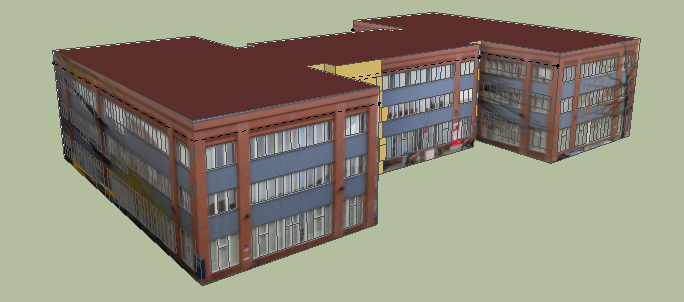
\includegraphics[width=0.8\textwidth]{phase1/group2/figures/kaiserin.png}
	\caption{Model of building located at Kaiserin-Augusta-Alle 10B}
	\label{fig:kaiserin}
\end{figure}


\subsection{Conclusion}
From the visualization of the results of the building model, it can be seen that the building model created had been used to replace the LoD 2 model, with this change the city gml model of berlin has been updated for four selected buildings to LoD 3 with useful energy attributes and generic attributes that can allowed for different query and simulations. The approach has seen compared to previous approach can be said to be cost effective and possible for implementation on small data set. This approach will not be suitable on large set of data because it might be very complicated and time consuming. It will be ideal to use this project approach for regular or periodic update of selected data or addition of new data of newly constructed building into the 3D cadastral. 




